\documentclass[../basic_graph_theory.tex]{subfiles}

\begin{document}
\chapter{Spectral Graph Theory}
\setcounter{chapter}{8} %Set chapter counter
\setcounter{section}{0}
\setcounter{equation}{0}
\setcounter{figure}{0}

This chapter employs linear algebra tools to systematically investigate graph properties, thereby facilitating a more lucid comprehension and expeditious validation of proofs for both antecedent and contemporary results.

\ssk

We start by clarifying our convention. For a graph $ G = (V, E) $ on $ n $ vertices and $ m $ edges, we denote the vertex set $ V(G) $ as $ [n] = \left\{ 1, \dots, n \right\} $ and the edge set $ E(G) $ as $ E = \left\{ e_{1}, \dots, e_{m} \right\} $. We will also assume that the vertices of $ G $ are ordered in some way.

\section{Basic facts from Linear Algebra}

\textit{\textbf{To be added...}}

\section{Incidence Matrix}

\begin{Def}{}{Incidence Matrix}
  Let $G$ be a graph with $n$ vertices and $m$ edges, we first assign an orientation to the edges and consider them as $E(G) = \left\{ e_j = \left( e_j^{+}, e_j^{-} \right) \mid j = 1, \dots, m \right\} $. Here, $ e_j^{+} $ denotes the vertex where the edge \(e_j\) is outgoing and $ e_j^{-} $ denotes the vertex where the same is incoming. Then the \textbf{incidence matrix} of $G$ is the $n \times m$ matrix $Q = \left( (q_{ij}) \right)_{m \times n}$ defined as follows:
  \begin{align*}
    q_{ij} = \begin{cases}
               1  & \text{if } v_{i} = e_{j}^{+} \\
               -1 & \text{if } v_{i} = e_{j}^{-} \\
               0  & \text{otherwise}
             \end{cases}
  \end{align*}
\end{Def}

\begin{figure}[hbt]
  \centering
  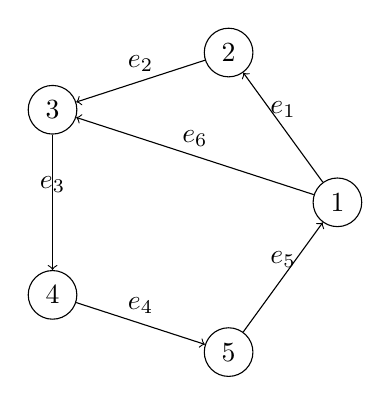
\begin{tikzpicture}[->]
    % Nodes
    \foreach \i in {1,...,5}
    \node[circle, draw, minimum size=5mm] (N\i) at ({360/5 * (\i - 1)}:2cm) {$\i$};

    % Edges
    \foreach \i/\j/\edgeindex in {1/2/1, 2/3/2, 3/4/3, 4/5/4, 5/1/5, 1/3/6}
    \draw (N\i) -> (N\j) node[midway, above] {$e_{\edgeindex}$};
  \end{tikzpicture}
  \label{fig:incidence}
  \caption{Graph $G_1 = \left( [5], \left\{ e_1, \dots, e_6 \right\}  \right)$}
\end{figure}

\begin{Eg}{}{incidence}
  Consider the graph $ G_1 $ having the incidence matrix $ Q(G_1) $ as follows:
  \[
    Q(G_1) = \begin{pmatrix}
      \ \ 1 & \ \ 0 & \ \ 0 & \ \ 0 & -1    & \ \ 1 \\
      -1    & \ \ 1 & \ \ 0 & \ \ 0 & \ \ 0 & \ \ 0 \\
      \ \ 0 & -1    & \ \ 1 & \ \ 0 & \ \ 0 & -1    \\
      \ \ 0 & \ \ 0 & -1    & \ \ 1 & \ \ 0 & \ \ 0 \\
      \ \ 0 & \ \ 0 & \ \ 0 & -1    & \ \ 1 & \ \ 0
    \end{pmatrix}
  \]
\end{Eg}

Now, we list some basic properties of the incidence matrix.
\begin{Thm}{}{}
  Consider a graph $G$ with $n$ vertices and $m$ edges. For two incidence matrices $ Q_1 $ and $ Q_2 $ of $ G $, there exists a diagonal matrix $ D $ of order \(m\) with diagonal entries \(\pm 1\) such that $ Q_1 = Q_2 D $.
\end{Thm}
\begin{proof}
  Considering the digraphs corresponding to \(Q_1\) and \(Q_2\), and noting their shared underlying graph with identical vertices and edges, we relabel the edges of \(Q_2\) to align with \(Q_1\). Define the diagonal matrix \(D\) such that \(D_{ii} = 1\) if the \(i^{\text{th}}\) edge has the same orientation in both \(Q_1\) and \(Q_2\), and \(D_{ii} = -1\) if their orientations are opposite. This establishes \(Q_1 = Q_2 D\), which completes the proof.
\end{proof}

So, it doesn't matter which orientation we choose for the edges of a graph, because every incidence matrix is the same up to the right multiplication of some \(\pm 1\) diagonal matrix.

\ssk

Next we investigate the rank of the incidence matrix. For a graph \(G\), note that the column sums of \(Q(G)\) are zero due to each edge being incident to exactly two vertices, and each vertex being incident to exactly two edges.

\begin{Thm}{Rank}{rank:incidence}
  If \(G\) is a connected graph on \(n\) vertices, then \(\rank Q(G) = n - 1\). More generally, if \(G\) has \(k\) components, then \(\rank Q(G) = n - k\).
\end{Thm}
\begin{proof}
  For a connected graph \(G\), let \(x\) be in the left null space of \(Q := Q(G)\), i.e., \(x^TQ = 0\). Since \(G\) is connected, all components of \(x\) are equal. Thus, the left null space of \(Q\) is at most one-dimensional, making the rank of \(Q\) at least \(n - 1\). Also, as the rows of \(Q\) are linearly dependent, \(\rank Q \leq n - 1\), implying \(\rank Q = n - 1\).

  If \(G\) has \(k\) connected components, after relabeling the vertices (if necessary), we can express \(Q(G)\) as a block diagonal matrix,
  \[
    Q(G) = \begin{pmatrix} Q(G_1) & & \\ & \ddots & \\ & & Q(G_k) \end{pmatrix}
  \]
  Since each \(G_i\) is connected, \(\rank Q(G_i) = n_i - 1\), where \(n_i\) is the number of vertices in \(G_i\). Thus, \(\rank Q = \rank Q_1 + \dots + \rank Q_k = n - k\).
\end{proof}

\begin{Thm}{}{column:independent}
  Let \(G\) be a graph on \(n\) vertices. Columns \(j_1, \dots, j_k\) of \(Q(G)\) are linearly independent if and only if the corresponding edges of \(G\) induce an acyclic subgraph.
\end{Thm}
\begin{proof}
  Consider edges \(j_1, \dots, j_k\) and suppose there is a cycle in the induced subgraph. Without loss of generality, suppose the columns \(j_1, \dots, j_p\) form a cycle. After relabeling vertices if needed, the submatrix of \(Q(G)\) formed by \(j_1, \dots, j_p\) is \(\begin{bmatrix} B \\ 0 \end{bmatrix}\), where \(B\) is the \(p \times p\) incidence matrix of the cycle. Since \(B\) is singular (having column sums zero), \(j_1, \dots, j_p\) are dependent, which proves the "only if" part.

  Conversely, if \(j_1, \dots, j_k\) induce an acyclic graph (a forest), and the forest has \(q\) components, then \(k = n - q\), which is the rank of the submatrix formed by \(j_1, \dots, j_k\) (by Theorem \ref{th:rank:incidence}). Therefore, the columns \(j_1, \dots, j_k\) are independent.
\end{proof}

Now we look at the square submatrices of the incidence matrix.

\begin{Def}{Totally unimodular matrix}{tum}
  A matrix is called \textbf{totally unimodular} if every square submatrix has determinant \(0, 1,\) or \(-1\).
\end{Def}

It can be easily proved by induction on the order of the submatrix that \(Q(G)\) is totally unimodular which is our next result.

\begin{Thm}{}{tum:incidence}
  Let \(G\) be a graph with incidence matrix \(Q(G)\). Then \(Q(G)\) is totally unimodular.
\end{Thm}
\begin{proof}
  We prove the statement that any \(k \times k\) submatrix of \(Q(G)\) has determinant \(0\) or \(\pm 1\) by induction on \(k\). For \(k = 1\), the statement is evident since each entry of \(Q(G)\) is either \(0\) or \(\pm 1\). Assuming the statement holds for \(k - 1\), consider a \(k \times k\) submatrix \(B\) of \(Q(G)\).

  If each column of \(B\) has a \(1\) and \(k - 1\) zeros, or if \(B\) has a zero column, then \( \det B = 0\). If \(B\) has a column with only one nonzero entry, which must be \(\pm 1\), expanding the determinant along that column and using the induction assumption implies that \(\det B\) must be \(0\) or \(\pm 1\).
\end{proof}

\begin{Thm}{}{}
  Let \(G\) be a tree on \(n\) vertices. Then any submatrix of \(Q(G)\) of order \(n - 1\) is nonsingular. Moreover, their determinant have the same absolute value.
\end{Thm}
\begin{proof}
  Consider any \(n - 1\) rows of \(Q(G)\), say \(1, 2, \dots, n - 1\), and let \(B\) be the submatrix formed by these rows. Let \(x\) be a row vector of \(n - 1\) components in the row null space of \(B\). As in the proof of Theorem \ref{th:rank:incidence}, \(x_i = 0\) whenever \(i \sim n\), and the connectedness of \(G\) implies \(x\) is the zero vector. Thus, the rank of \(B\) is \(n - 1\), making \(B\) nonsingular.

  \ssk

  Consider,
  \begin{align*}
    \det B = \det \begin{pmatrix}
                    v_1 \\ v_2 \\ \vdots \\ v_{n-1}
                  \end{pmatrix}
    = \det \begin{pmatrix}
             -\sum_{j = 2}^{n} v_j \\ v_2 \\ \vdots \\ v_{n-1}
           \end{pmatrix}
    = \det \begin{pmatrix}
             -v_n \\ v_2 \\ \vdots \\ v_{n-1}
           \end{pmatrix}
    = \det \begin{pmatrix}
             v_2 \\ \vdots \\ v_{n-1} \\ v_n
           \end{pmatrix}
  \end{align*}
  It's your job to convince yourself, no matter which \(n - 1\) rows we choose, the determinant of the corresponding submatrix remains the same (upto sign).
\end{proof}

\section{Adjacency Matrix}

\begin{Def}{}{Adjacency Matrix}
  For a graph $G$ with verices $V(G) = [n]$ and edges $E(G) = \left\{ e_1, \dots, e_m \right\}$, the \textbf{adjacency matrix} of $G$ is the $n \times n$ matrix $A = (a_{ij})$ defined as follows:
  \begin{align*}
    a_{ij} = \begin{cases}
               1 & \text{if } \{i, j\} \in E(G) \\
               0 & \text{otherwise}
             \end{cases}
  \end{align*}
\end{Def}

\begin{figure}[ht]
  \centering
  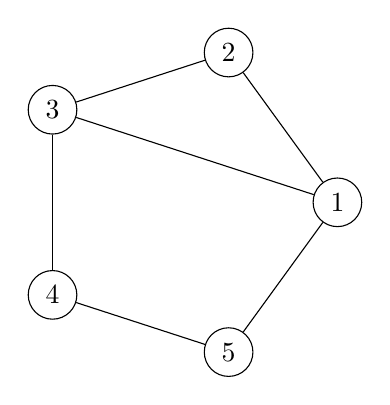
\begin{tikzpicture}
    % Nodes
    \foreach \i in {1,...,5}
    \node[circle, draw, minimum size=5mm] (N\i) at ({360/5 * (\i - 1)}:2cm) {$\i$};

    % Edges
    \foreach \i/\j in {1/2, 2/3, 3/4, 4/5, 5/1, 1/3}
    \draw (N\i) -- (N\j);
  \end{tikzpicture}
  \label{fig:adjacency}
  \caption{Graph $G_2$}
\end{figure}

\begin{Eg}{}{adjacency}
  Consider the graph $ G_2 $ as undirected version of \(G_1\). It has the adjacency matrix $ A(G_2) $ as follows:
  \[
    A(G_2) = \begin{pmatrix}
      0 & 1 & 1 & 0 & 1 \\
      1 & 0 & 1 & 0 & 0 \\
      1 & 1 & 0 & 1 & 0 \\
      0 & 0 & 1 & 0 & 1 \\
      1 & 0 & 0 & 1 & 0
    \end{pmatrix}
  \]
\end{Eg}

\begin{Thm}{}{}
  Let \(G\) be a connected graph with vertices \([n]\) and let \(A\) be the adjacency matrix of \(G\). The \((i,j)^{\text{th}}\) entry \(a_{ij}^k\) of \(A^k\) counts the number of \(k\)-length walks with starting and end vertices \(i\) and \(j\) respectively.
\end{Thm}
\begin{proof}
  By induction on \(k\), the result is evident for \(k = 1\). Assuming it holds for \(k = m\), consider \(A^{m+1} = A^m A\). By induction hypothesis, \((i,j)\)-th entry of \(A^m\) counts walks of length \(m\) between vertices \(i\) and \(j\). Now, the number of walks of length \(m + 1\) between \(i\) and \(j\) equals the walks of length \(m\) from \(i\) to each vertex \(k\) adjacent to \(j\). This is expressed as
  \[
    \sum_{k \sim j} a_{ik}^m = \sum_{k = 1}^{n} a^m_{ik} a_{kj} = a_{ij}^{m+1}
  \]
  which is precisely the \((i,j)^{\text{th}}\) entry of \(A^{m+1} = A^m A\). Hence, the result follows.
\end{proof}

\begin{Thm}{}{}
  Let \(G\) be a connected graph with vertices \([n]\) and let \(A\) be the adjacency matrix of \(G\). If \(i, j\) are vertices of \(G\) with \(d(i, j) = m\), then the matrices \(I, A, \dots, A^m\) are linearly independent.
\end{Thm}
\begin{proof}
  We may assume \(i \not= j\). There is no \((ij)\)-path of length less than \(m\). Thus, the \((i, j)\)-element of \(I, A, \dots, A^{m-1}\) is zero, whereas the \((i, j)\)-element of \(A^m\) is nonzero. Hence, the result follows.
\end{proof}

\subsection*{Eigenalues of some graphs}

\begin{tcolorbox}[breakable]
  \textbf{Complete grpah}, \(K_n\). \(\big\{ n - 1, \underbrace{-1, \dots, -1}_{n - 1} \big\}\)

  \ssk

  Since every vertex of \(K_n\) is adjacent to every other vertex, the adjacency matrix consists of all ones except the diagonal entries, which are zero. Thus \(A(K_n) = J_n - I_n\), where \(J_n\) is the matrix of all ones and \(I_n\) is the identity matrix of order \(n\).

  Recall that \(P_n = \frac{J_n}{n}\) is the projection matrix onto the subspace spanned by the all ones vector. And note that the identity matrix \(I_n\) can be decomposed as the direct sum of \(P_n\) and \(P_n^{\perp}\), which is the projection matrix of it's complement subspace, i.e. \(I_n = P_n + P_n^{\perp}\). Thus
  \begin{align*}
    A(K_n)
     & = J_n - I_n                  \\
     & = nP_n - (P_n + P_n^{\perp}) \\
     & = (n-1)P_n + (-1)P_n^{\perp}
  \end{align*}
  which is obviously the spectral decomposition of \(A(K_n)\). So the eigenvalues of \(A(K_n)\) are \(n-1\) with multiplicity \(\rank P_n = 1\) and \(-1\) with multiplicity \(n - \rank P_n = n-1\).
\end{tcolorbox}

\begin{tcolorbox}[breakable]
  \textbf{Complete Bipartite grpah}, \(K_{p, q}\). \(\big\{ \sqrt{pq}, -\sqrt{pq}, \underbrace{0, \dots, 0}_{p + q - 2} \big\}\).

  \ssk

  Note that,
  \[A(K_{p, q}) = \begin{pmatrix}
      0        & J_{p, q} \\
      J_{q, p} & 0
    \end{pmatrix}\]
  where \(J_{p, q}\) is the \(p \times q\) matrix of all ones. Since both \(J_{p, q}\) and \(J_{q, p}\) have rank \(1\), \(\rank A(K_{p, q}) = 2\), yielding \(0\) as an eigenvalue with multiplicity \(p + q - 2\).
  Let \(\lambda\) be a non-zero eigenvalue of \(A\) with an eigenvector \(v = \begin{pmatrix} x \\ y \end{pmatrix}\). Now, \(A(K_{p, q})v = \lambda v\) implies \(J_{p, q}y = \lambda x\) and \(J_{q, p}x = \lambda y\). So \(qJ_px = \lambda^2 x\). Since \(J_p\) has the eigenvalue \(p\) with multiplicity \(1\) and \(0\) with multiplicity \(p - 1\), and \(\lambda \neq 0\), we get \(\lambda^2 = pq\), which gives \(\lambda = \pm \sqrt{pq}\). So the eigenvalues of \(A(K_{p, q})\) are \(0\) with multiplicity \(p + q - 2\) and \(\pm \sqrt{pq}\) each with multiplicity \(1\).
\end{tcolorbox}

\begin{tcolorbox}[breakable]
  \textbf{Cycle graph}, \(C_n\). \(\left\{ 2\cos{\frac{2\pi k}{n}} \mid k = 1, \dots, n \right\}\).

  \ssk

  Note that,
  \[ A(C_n) = U_n + U_n^{T} \]
  where \(U_n\) is the upshift matrix of order \(n\), and \(U_n U_n^T = I_n = U_n^T U_n\). Utilizing the eigenvalues of \(U_n\), given by \(\left\{ \omega^k \mid k = 1, \dots, n \right\}\) where \(\omega\) is the \(n^{\text{th}}\) root of unity, we obtain that the eigenvalues of \(A(C_n)\) are \(\left\{ \omega^k + \omega^{n-k} \mid k = 1, \dots, n \right\}\).
\end{tcolorbox}

\begin{Def}{Elementary Subgraph}{elemsubg}
  Let \(G\) be a graph with \(V(G) = [n]\). A subgraph \(H\) of \(G\) is called an spanning elementary subgraph if each connected component of \(H\) is either an edge or a cycle.
\end{Def}

We will denote \(c(H)\) and \(c_1(H)\) as the number of components of \(H\) which are edges and cycles respectively.

\begin{Thm}{Determinant}{det:adj}
  Let \(G\) be a graph with vertices \([n]\) and adjacency matrix \(A\). Then
  \[
    \det A = \sum_{\substack{H \subseteq G \\ \text{spanning} \\ \text{elementary}}} (-1)^{n - c_1(H) - c(H)} 2^{c(H)}
  \]
\end{Thm}

\section{Laplacian}

For a graph $G$ with $n$ vertices and $m$ edges, the \textbf{Laplacian matrix} of $G$ is the $n \times m$ matrix $L$ defined as \(L = QQ^T\)

\ssk

\textit{\textbf{To be added...}}

\end{document}